\documentclass{vldb}
\usepackage{graphicx}
\usepackage{balance}  % for  \balance command ON LAST PAGE  (only there!)
\usepackage{bnf}
\usepackage{listings}
\usepackage{algorithm}

\newcommand{\remove}{}
\newcommand{\old}[1]{}
\newcommand{\match}{\stackrel{M}{=}}
\newcommand{\ncite}[1]{$^{\mbox{\tiny \citep{#1}}}$}
%\newcommand{\nncite}[1]{\citep{#1}}
\newcommand{\frags}{{\cal F}}
\newcommand{\snips}{{\cal S}}
\newcommand{\A}{{\tt A}}
\newcommand{\B}{{\tt B}}
\newcommand{\gap}{{\tt -}}
\newcommand{\ideas}{\vskip 0.6cm {\bf IDEAS:\ }}
\newcommand{\motivation}{\vskip 0.6cm {\bf MOTIVATION:\ }}
\newcommand{\mcost}[2]{#1 #2}
\newcommand{\ali}{$\mbox{ }$\hspace{0.2in}}
\newcommand{\acomment}[1]{\hspace{1in}\#{\em #1}}
\newcommand{\beqn}{\begin{equation}}
\newcommand{\eeqn}{\end{equation}}
\newcommand{\captionsize}{\footnotesize}
\newcommand{\LtoN}[1]{\parallel #1 \parallel_{2}}
\newcommand{\mecca}{HapCUT$\:$}

\newcommand{\Reads}{\ensuretext{{\sc Reads}}}
\newcommand{\AlignStr}{\ensuretext{{\sc AlignStr}}}
\newcommand{\Intervals}{\ensuretext{{\sc Intervals}}}
\newcommand{\Strand}{\ensuretext{{\sc Strand}}}
\newcommand{\Partner}{\ensuretext{{\sc Partner}}}
\newcommand{\MST}{\ensuremath{\mathit{MST}}}
\newcommand{\dist}{\ensuremath{\mathit{dist}}}
\newcommand{\TG}[2]{\ensuremath{\mathit{#1}^{(#2)}}}
\newcommand{\CC}{\ensuremath{\mathcal{CC}}}
\newcommand{\psubs}{\stackrel{\subset}{+}}
\newcommand{\rs}{\ensuremath{\mathit{R_s}}}
\newcommand{\MEC}{\ensuremath{\mathit{MEC}}}
\newcommand{\Prob}{\ensuremath{\mbox{Pr}}}
\newcommand{\fref}[1]{\mbox{Figure~\ref{#1}}}
\newcommand{\secref}[1]{\mbox{Section~\ref{#1}}}
\newcommand{\algref}[1]{\mbox{Algorithm~\ref{#1}}}
\newcommand{\para}[1]{\vspace{2pt}\noindent\mbox{{\bf #1:} }}
\newcommand{\slimfast}{{\sc SlimGene}}

%%%%%%%%%%%%%%%%%%%%%%%%%%%%%%%%
% GenomeQL syntax
%%%%%%%%%%%%%%%%%%%%%%%%%%%%%%%%%%%
\newcommand{\MapRel}{\ensuremath{\:\overline{\bowtie}\:}}
%\newcommand{\MapRel}{\ensuremath{\stackrel{\bowtie}{\llcorner\lrcorner}}}
\newcommand{\NatJoin}{\ensuremath{{\bowtie}}}
%\newcommand{\MapRel}{\ensuremath{\bowtie_M}}
\newcommand{\Project}[1]{\ensuremath{\Pi_{#1}}}
\newcommand{\ProjectInterval}[1]{\ensuremath{\Pi^i_{#1}}}
\newcommand{\Select}[1]{\ensuremath{{\displaystyle \sigma_{#1}}}}

\newcommand{\gqlSelect}{{\sc select}}
\newcommand{\gqlFrom}{{\sc from}}
\newcommand{\gqlWhere}{{\sc where}}
\newcommand{\gqlAnd}{{\sc and}}
\newcommand{\gqlAvg}{{\sc avg}}
\newcommand{\gqlMin}{{\sc min}}
\newcommand{\gqlMax}{{\sc max}}
\newcommand{\gqlIn}{{\sc in}}
\newcommand{\gqlAbs}{{\sc abs}}
\newcommand{\gqlCount}{{\sc count}}
\newcommand{\gqlGroupby}{{\sc groupby}}
\newcommand{\gqlIntersects}{{\sc intersect}}
\newcommand{\gqlMapjoin}{{\sc mapjoin}}
\newcommand{\gqlProjectInterval}{\gqlSelect\ {\sc merged}}

\newenvironment{packed_enum}{
\begin{enumerate}
  \setlength{\itemsep}{1pt}
  \setlength{\parskip}{0pt}
  \setlength{\parsep}{0pt}
}{\end{enumerate}}
\newenvironment{packed_itemize}{
\begin{itemize}
  \setlength{\itemsep}{1pt}
  \setlength{\parskip}{0pt}
  \setlength{\parsep}{0pt}
}{\end{itemize}}


\lstdefinelanguage{genomeql}{
	morekeywords={using, use, import, select, from, where, mapjoin,
	both\_mates, and, or, not, (, ), <, =, ==, >, !=, >=, <=,
	READS[2], interval\_creation[2], interval\_coverage[2]},
	sensitive=false,
	morecomment=[l]{\#},
	morestring=[b]",
	morestring=[b]',
}

\lstset{language=genomeql}

\begin{document}

% ****************** TITLE ****************************************

\title{Abstractions for Genomics: Or, which way to the Genomic Information Age?
}

% ****************** AUTHORS **************************************

% You need the command \numberofauthors to handle the 'placement
% and alignment' of the authors beneath the title.
%
% For aesthetic reasons, we recommend 'three authors at a time'
% i.e. three 'name/affiliation blocks' be placed beneath the title.
%
% NOTE: You are NOT restricted in how many 'rows' of
% "name/affiliations" may appear. We just ask that you restrict
% the number of 'columns' to three.
%
% Because of the available 'opening page real-estate'
% we ask you to refrain from putting more than six authors
% (two rows with three columns) beneath the article title.
% More than six makes the first-page appear very cluttered indeed.
%
% Use the \alignauthor commands to handle the names
% and affiliations for an 'aesthetic maximum' of six authors.
% Add names, affiliations, addresses for
% the seventh etc. author(s) as the argument for the
% \additionalauthors command.
% These 'additional authors' will be output/set for you
% without further effort on your part as the last section in
% the body of your article BEFORE References or any Appendices.

\numberofauthors{5} %  in this sample file, there are a *total*
% of EIGHT authors. SIX appear on the 'first-page' (for formatting
% reasons) and the remaining two appear in the \additionalauthors section.

\author{
% You can go ahead and credit any number of authors here,
% e.g. one 'row of three' or two rows (consisting of one row of three
% and a second row of one, two or three).
%
% The command \alignauthor (no curly braces needed) should
% precede each author name, affiliation/snail-mail address and
% e-mail address. Additionally, tag each line of
% affiliation/address with \affaddr, and tag the
% e-mail address with \email.
%
% 1st. author
\alignauthor
Christos Kozanitis \titlenote{Corresponding author}\\
       \affaddr{Computer Science and Engineering}\\
       \affaddr{UC San Diego}\\
       \email{ckozanit@ucsd.edu}
% 2nd. author
\alignauthor Alin Deutsch \\
       \affaddr{Computer Science and Engineering}\\
       \affaddr{UC San Diego}\\
% 3rd. author
\alignauthor Andrew Heiberg \\
       \affaddr{Computer Science and Engineering}\\
       \affaddr{UC San Diego}\\
\and  % use '\and' if you need 'another row' of author names
% 4th. author
\alignauthor Vineet Bafna\\
       \affaddr{Computer Science and Engineering}\\
       \affaddr{UC San Diego}\\
% 5th. author
\alignauthor George Varghese\\
       \affaddr{Computer Science and Engineering}\\
       \affaddr{UC San Diego}\\
}
% There's nothing stopping you putting the seventh, eighth, etc.
% author on the opening page (as the 'third row') but we ask,
% for aesthetic reasons that you place these 'additional authors'
% in the \additional authors block, viz.
%\additionalauthors{Additional authors: John Smith (The Th{\o}rv\"{a}ld Group, {\texttt{jsmith@affiliation.org}}), Julius P.~Kumquat
%(The \raggedright{Kumquat} Consortium, {\small \texttt{jpkumquat@consortium.net}}), and Ahmet Sacan (Drexel University, {\small \texttt{ahmetdevel@gmail.com}})}
%\date{30 July 1999}
% Just remember to make sure that the TOTAL number of authors
% is the number that will appear on the first page PLUS the
% number that will appear in the \additionalauthors section.


\maketitle

\begin{abstract}
The abstract for your paper for the PVLDB Journal submission.
The template and the example document are based on the ACM SIG Proceedings  templates. This file is part of a package for preparing the submissions for review. These files are in the camera-ready format, but they do not contain the full copyright note.
Note that after the notification of acceptance, there will be an updated style file for the camera-ready submission containing the copyright note.
\end{abstract}




\section{Introduction}
\label{sec:intro}

\section{Software Layering for Genomics}
\label{sec:layering}

\section{Software layers and interfaces for  genomics (from cacm)}
\label{sec:vision}
Our vision is inspired by analogy with systems and networks, where
software layering has solved similar problems. For example, the
Internet has successfully dealt with a wide variety of new link
technologies (from dialup to wireless) and applications (from email to
social networks) via the ``hourglass'' model using the key
abstractions of TCP and IP (Figure~\ref{fig:abstraction}a). 

In the same way, we propose that Genomic Processing software be
layered into an instrument layer, a compression layer, an evidence
layer, an inference layer, and a variation layer that can insulate
genomic applications from sequencing technology. Note that the only
way to achieve such modularity is to forgo some possible efficiencies
that could be gained by leaking information across layers.  For
example, biological inferences can be sharpened by considering which
sequencing technology is being used (e.g., Illumina versus Life
Technologies) but we suggest that modularity is paramount.

Some of the initial interfaces are already in vogue with standard
formats for exchange. Many instruments now produce sequence data as
`fastq' format; The output of mapping reads is often represented as
SAM/BAM format~\cite{sambam}, although other compressed formats are
coming into vogue~\cite{Kozanitis2011}.  At the highest level, there exists
standard such as VCF~\cite{VCF} to describe variants in a standardized way.  The existing
formats are shown bolded in Figure~\ref{fig:abstraction}a)

Here, we propose additional
layering between the mapped tools and applications. Specifically, we
separate the collection of \emph{evidence} required to support a query
(deterministic, large data movement, standardized) from the
\emph{inference} (probabilistic, comparatively smaller data movement,
little agreement on techniques).

We show that the Evidence Layer (EL) can be implemented on a compute
cloud while the more volatile Inference Layer can be implemented on
the desktop.  We assert that while Inference methods vary
considerably, the Evidence for inferences is fairly standard and hence
propose a Genome Query Language (GQL) that permits efficient
implementation, and presents a flexible mechanism for gathering
evidence for Inference.

Note that while we focus on the Evidence-Inference layer in this
paper, a careful specification of a variation layer
(Figure~\ref{fig:abstraction}a)) is also important.  While the data
format of a variation is standardized using, for example,
VCF~\cite{VCF}, the interface functions are not.  An application like
personalized medicine or discovery will query the variation layer and
join the variation information with phenotype information gleaned from
medical records (EMRs).

\begin{figure}[h!]
  \centering
 (a) 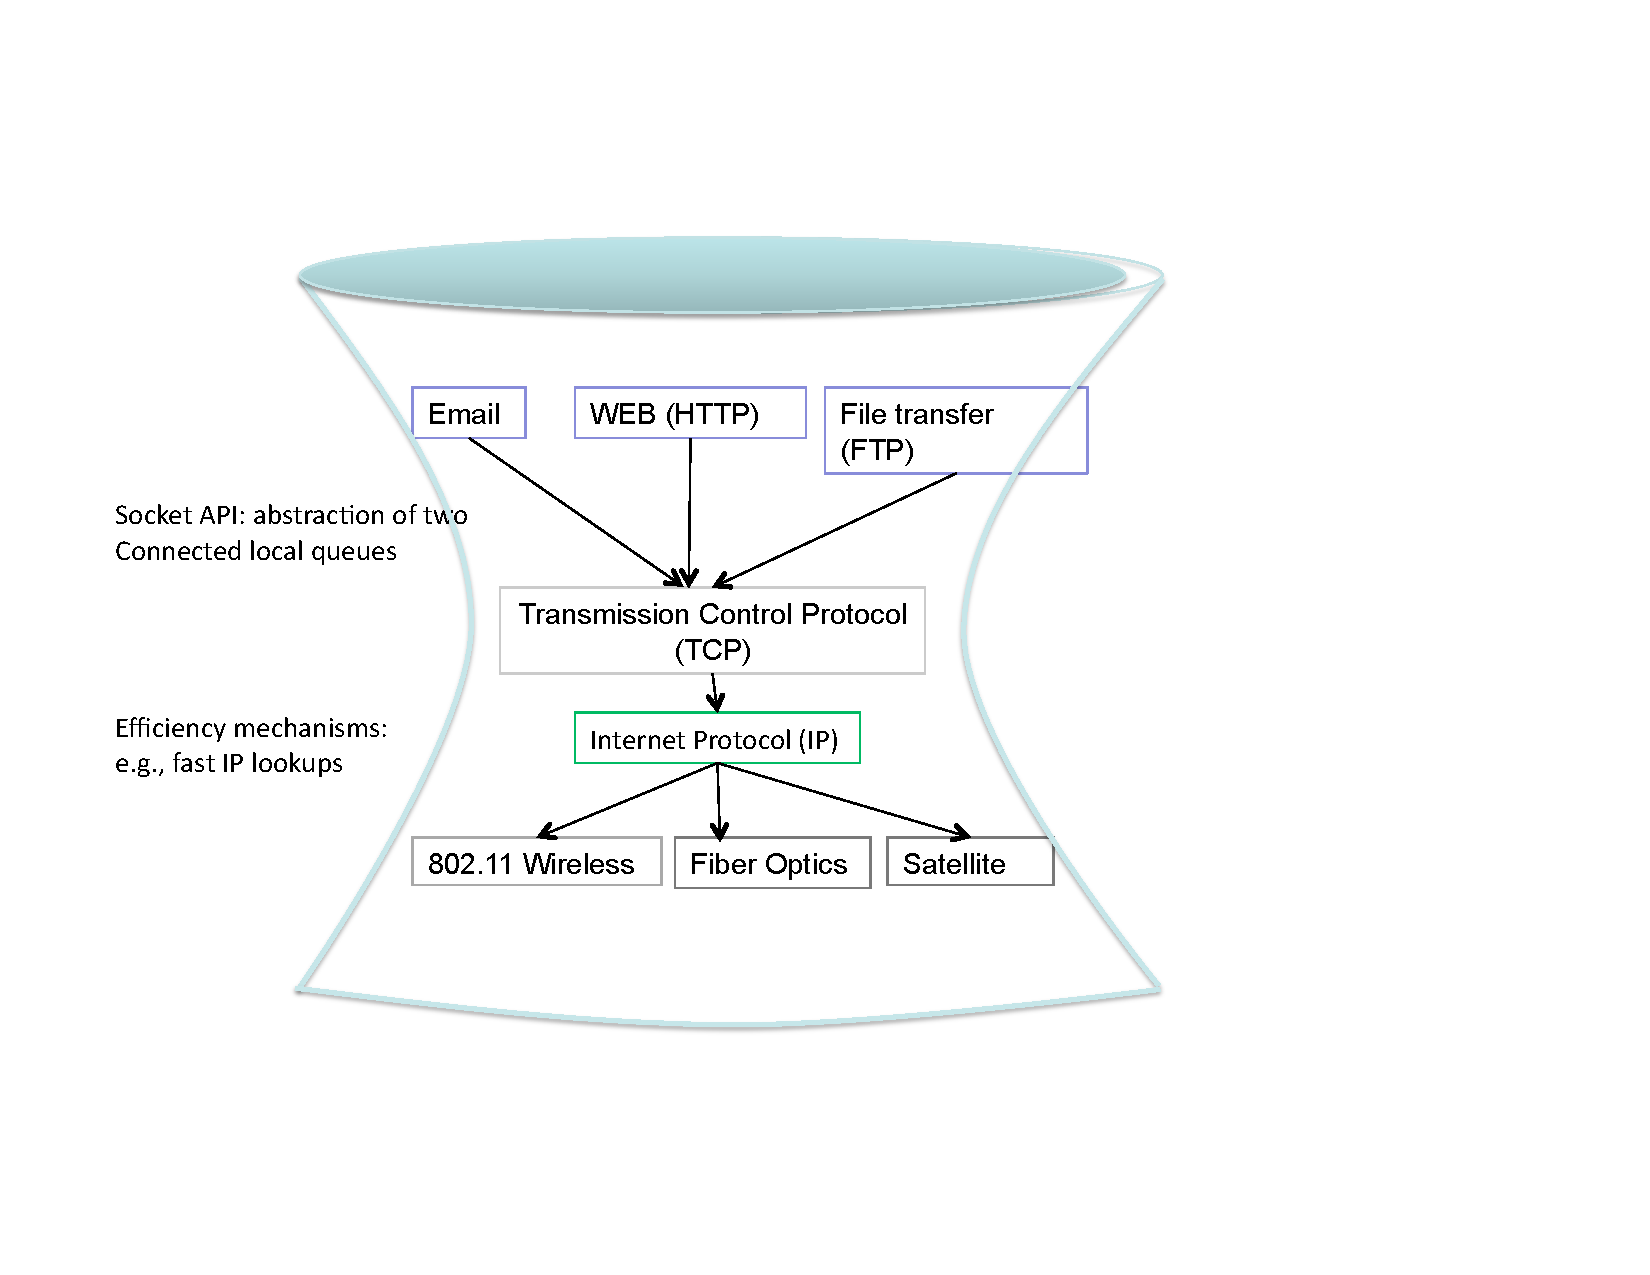
\includegraphics[trim = 0mm 40mm 60mm 10mm, clip, width=2.0in]{fig/hourglass.pdf}
  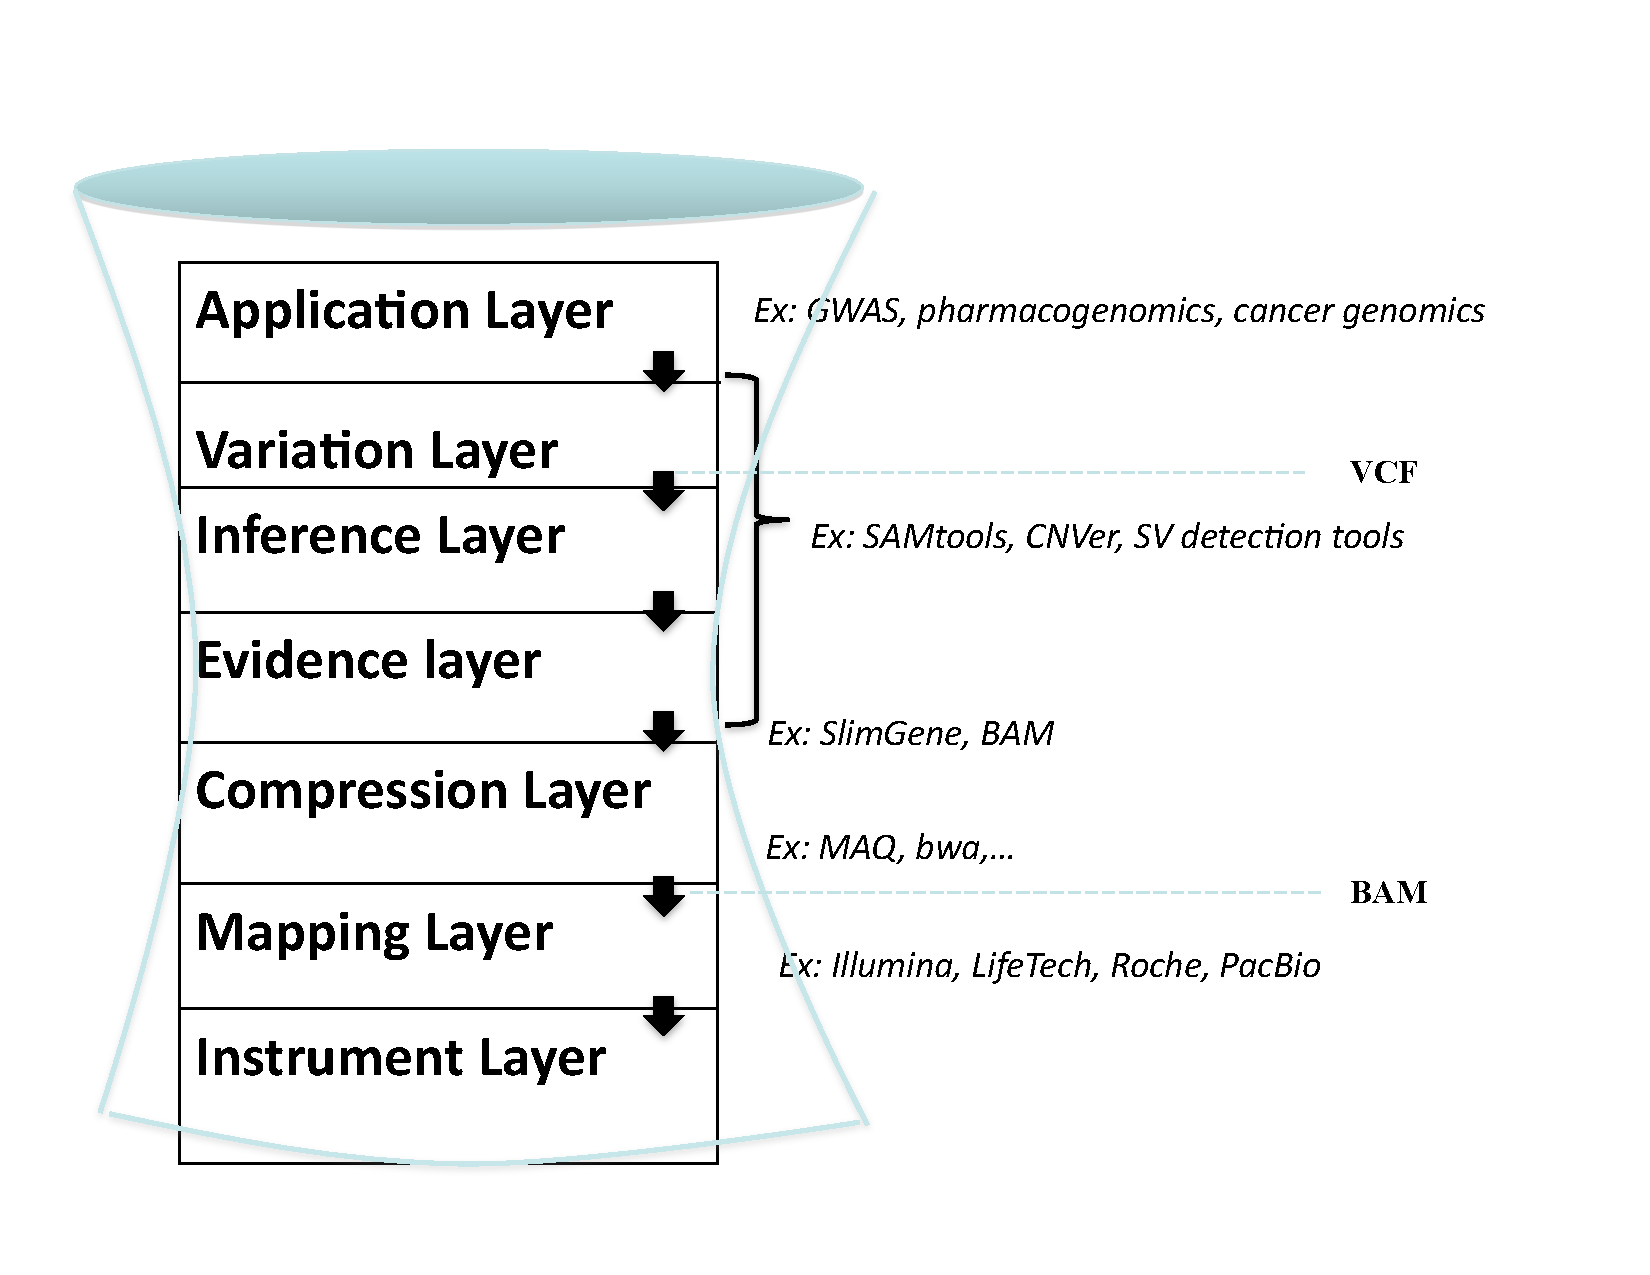
\includegraphics[trim = 0mm 15mm 40mm 10mm, clip, width=1.8in, height=1.8in]{fig/genomicabstraction.pdf}\\
 (b) 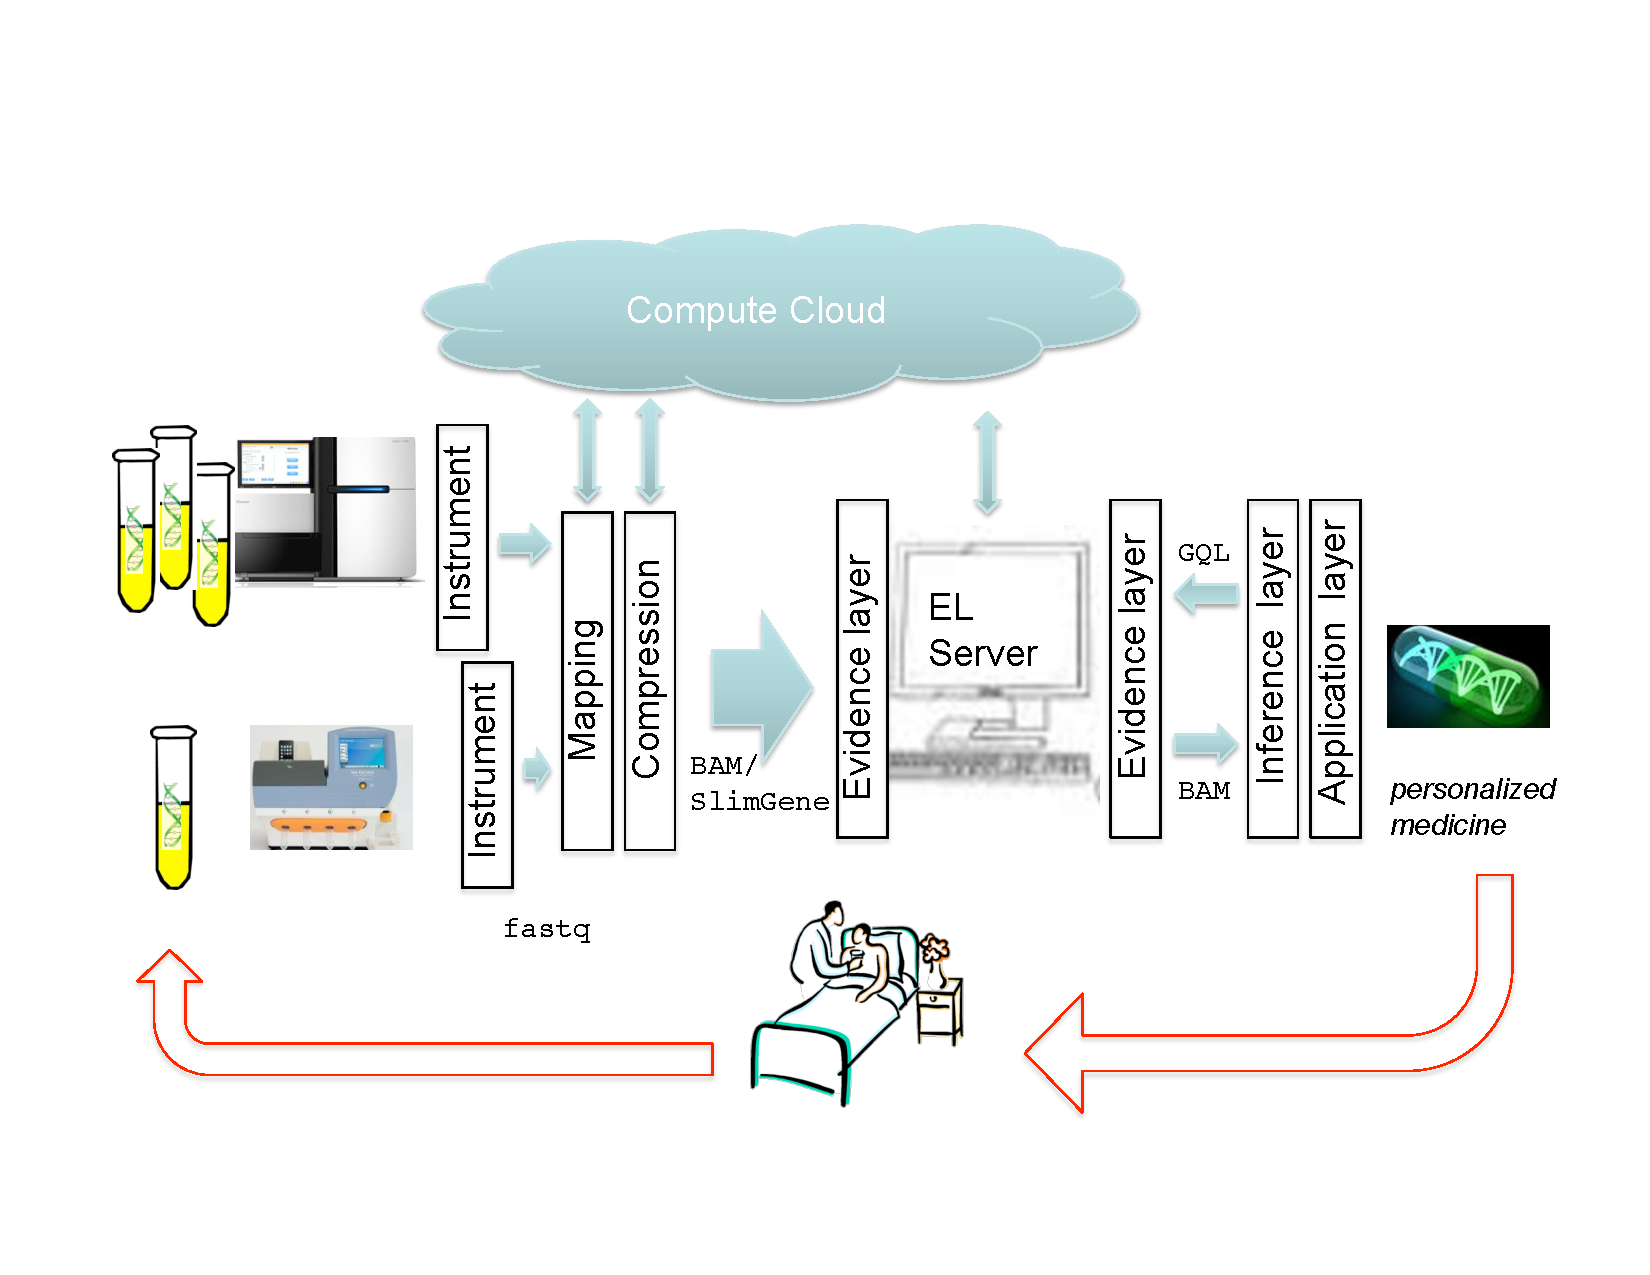
\includegraphics[trim = 20mm 20mm 10mm 30mm, clip, width=2.5in]{fig/vision.pdf}
 \caption{Abstraction for genomics. }
  \label{fig:abstraction}
\end{figure}
\subsection{The case for an evidence layer}
Consider a complex biological query: `` identify all deletions that
disrupt genes in a certain biological network, and the frequency of
those deletions in a natural population''. The bioinformatician
struggles to transfer this question into a problem of statistical
inference with bounds on false-positive and false-negative
errors. However, the first part of any such query would be the
gathering of the evidence. Here, the evidence would consist of all
reads, and their mappings that satisfy certain properties. For
example, the reads must overlap regions encoding genes in the given
biological network, and must fall in one of three categories: (a)
Concordantly mapping reads as these reads suggest heterozygosity of
the deletion; (b) discordant reads: all reads where the read and its
pair map to locations much further apart than could be explained by
natural variation in insert length, indicating a deletion in the
donor; (c) reads in which only one of the two ends are mapped, and
which are proximal to discordant reads, corresponding to reads that
map at the boundary of the deletion breakpoint. The development of an
EL to support such queries provides several advantages

\begin{packed_itemize}

\item The separation allows Inference Layer designers to start
  thinking of alternate forms of evidence to improve the confidence of
  their queries.  For example, we might consider looking for
  "partially mapped" READs.  If one pair of READs overlaps the
  boundary of a deletion, then that READ will match a prefix or suffix
  of the reference and the other may match perfectly.  If the mapping
  shows that one maps correctly and the second does not, it provides
  some evidence as to the location of the boundary; further a small
  amount of effort can be used to decide if the non-mapped pair has a
  partial match with the reference.

\item The EL often poses a `data bottleneck' as it involves sifting
  through large sets of genomic reads. By contrast, the inference
  layer may be compute intensive, but typically works on smaller
  amounts of data (filtered by the evidence layer). We can implement
  EL on the cloud while the Inference Layer can be implemented either
  on the cloud or on client workstations. The evidence can easily be
  transported across the network interactively (Mbytes versus
  Gbytes). We have already seen moves by commercial cloud operators
  like Amazon to host the 1000 genome data sets on their
  infrastructure.  The cloud allows rented computation on demand
  without the cost of maintaining a permanent cluster by every
  genomics researcher.

\item The standardization of the EL will allow vendors time to
  creating a fast and scalable EL implementation.  It is hard to do
  with the Inference Layer today as it is a moving target.
\end{packed_itemize}
In the following, we develop this intuitive idea further by describing a Genome
Query Language to support the Evidence Layer.

\section{GQA: a relational algebra for genome queries(from cacm)}
\label{sec:gqa}
\newcommand{\attr}{\ensuremath{\mathit{attr}}}
\newcommand{\ID}{\ensuremath{\mathit{ID}}}
\newcommand{\GrpBy}[2]{\ensuremath{_{#1}\Gamma_{#2}}}
\newcommand{\alin}[1]{{\small\bf [[[{#1} --alin]]]}}

We show that we can express most genomic queries in a relational
algebra (the \emph{Genome Query Algebra-GQA}, as also an SQL-like
language (the \emph{Genome Query Language-GQL}). While our syntax is
SQL-like, we need some special operators and relations that may not
fit with available Relational Database Management Systems (RDBMS). In
parallel, we are developing a database system to archive genomes and
support genomic queries.

Our database has some key relations. The first is \emph{R (Reads)}
that describe the set of read fragments output by the sequencer, and
all of their properties.  For example, for paired-end sequencing, $R$
could contain identifiers for each read $r$, and its paired-end. A
second relation encodes a set of intervals on the genome, where each
is specified by the triple ``$\langle\mbox{chromosome, start-position,
  end-position} \rangle$''. A specific, and important, case of the
interval relation is the relation $G$ (the genome) where each entry is
a point interval corresponding to a specific location ({\em locus })
on the genome. As $G$ is large ($3\cdot 10^9$ loci), we do not
materialize $G$ explicitly, using it instead as a virtual (conceptual)
relation to facilitate the relational expression of queries. A final
relation $P$ describes the set of all individuals in a population, and
will be discussed in a subsequent section.


As shown below, the key benefit of our proposed relational modeling is
to enable manipulation via algebraic operators (the standard
relational algebra operators, as well as domain-specific operators
defined shortly). This in turn creates the opportunity to leverage
proven techniques developed by the data management community for
efficiently querying large collections of data. Regardless of the fact
that some of these techniques need to be adapted or extended to our
specific domain, while others can be applied directly, the overarching
contribution here is to unlock the potential of large-scale data
processing in the context of a huge data scale challenge.



\paragraph{Standard relational algebra operators and language
  constructs}
Standard algebraic operators we use in the examples below include: 
\begin{packed_itemize}
\item The projection operator $\Project{}$ where $\Project{X}(E)$
  returns, from the relation $E$ evaluates to, the restriction of the
  tuples to the attributes named in $X$. In GQL, we express this
  operation using
  \[
  \mbox{\gqlSelect\ } \mbox{X}  \mbox{ \gqlFrom\ }  E
  \]
\item The selection operator $\Select{}$, where $\Select{\theta}(E)$
  selects the subset of precisely those tuples in the result of
  expression $E$ that satisfy filter predicate
  $\theta$. Correspondingly, in GQL:
  \[
  \mbox{\gqlSelect\ * \gqlFrom\  E \gqlWhere\ } \theta
  \]
\item The Cartesian product operator $\times$, where $E\times F$
  refers to all tuples of the form $(e,f)$ where $e\in E, f\in F$. In
  GQL:
  \[
    \mbox{\gqlSelect\ * \gqlFrom\  E,F}
  \]

\item The renaming operator $\rho_N(E)$, which sets to $N$ the name of
  the relation returned by $E$.
\item The group-by operator $\GrpBy{}{}$, where in
  \begin{displaymath}\GrpBy{G_1,G_2,\ldots,G_k}{N_1:F_1(A_1),\ldots,N_l:F_l(A_l)}(E)\end{displaymath},
  $E$ is an algebraic expression that evaluates to a relation,
  $G_1,\ldots,G_k$ are group-by attributes, each $F_i$ is an aggregate
  function and each $N_i,A_i$ are attribute names.  The meaning of the
  group-by operator is the standard one: all tuples in the result of
  $E$ are partitioned into groups, such that two tuples are in the
  same group if and only if they agree on the values of all group-by
  attributes.  Thus, the groups can be identified by the value of the
  group-by attributes.  For each group $(g_1,\ldots,g_k)$, the result
  contains a tuple of attributes $G_1,\ldots,G_k,N_1,\ldots,N_l$ and
  values \begin{displaymath}(g_1,\ldots,g_k,n_1,\ldots,n_l)\end{displaymath}, respectively. Here, each
  $n_i$ is computed by applying function $F_i$ to the collection of
  attribute $A_i$'s values found in the group. In GQL:
\[
  \begin{array}{l}
    \mbox{\gqlSelect\ }
	G_1,\ldots,G_k,N_1=F_1(A_1),\ldots,N_l=F_l(A_l) \\
	\mbox{\gqlFrom\ }  E\\ 
    \mbox{\gqlGroupby\ } G_1,\ldots G_k
  \end{array}
\]



By default, this
  collection is viewed as a multiset, i.e. duplicate values are not
  removed.  To apply $F_i$ after eliminating duplicates, we use the
  syntax \begin{displaymath}N_i:F_i(\mbox{distinct\ } A_i)\end{displaymath}.  The syntax of the count
  aggregation is an exception, in that no $A_i$ attribute need be
  specified.
\end{packed_itemize}

\paragraph{The Map join and the Project Interval operator}
As reads are sequenced, they are also mapped to the reference genome
using various mapping algorithms. Some mapping algorithms map each
read to a unique location, or not at all; others may choose to
identify all intervals where the underlying genomic string is similar
(in terms of edit distance) to the read. For now, assume that each
read is mapped to its best location by a mapping algorithm $M$, and
the relation $R$ includes the interval of the best map.


For an arbitrary relation of genomic intervals, $A$, define a
\emph{map-join} operation $R\MapRel A$ by a pair of tuples $(r,a)\in
R\times A$ such that (r.chr, r.start, r.end) and (a.chr, a.start,
a.end) `intersect'. Recall that we defined the relation $G$ as the set
of all genomic loci. Therefore, $R\MapRel G$, denotes the set of all
tuples $r,g$ where $g$ denotes a genomic coordinate that $r$ maps to.
In GQL:
\[
    \mbox{\gqlSelect\ } * \mbox{ \gqlFrom\ \gqlMapjoin\ }  R,G\\ 
\]


In many practical instances, the relation is quite large. If 33\% of
the genome was mapped on the average by 10 reads, $R\MapRel G$ would
contain $\simeq \frac{1}{3} 3\cdot 10^9\cdot 10= 10^{10}$ tuples.
To reduce output size, we define a special \emph{Project-interval}
operator $\ProjectInterval{}$. $\ProjectInterval{A.ID} (R\MapRel A)$
outputs all genomic intervals after `fusing' adjacent and overlapping
intervals. Thus,
\[
\ProjectInterval{G.ID} (R\MapRel G)
\] 
would result in the set of all disjoint genomic intervals with some
read mapping to them. Correspondingly, in GQL:
\[
    \mbox{\gqlProjectInterval\ G.ID} \mbox{ \gqlFrom\ \gqlMapjoin\ }  R,G\\ 
\]
We show, mostly by example, that a large corpus of biological queries
can be supported by these abstractions.


\section{Implementation}
\label{sec:impl}
This section introduces our indexing scheme and demonstrates its
capabilities by describing the implementation of a series of important
abstractions. \secref{sec:indx} describes our indexing,
\secref{sec:range} describes the range retrieval query,
\secref{sec:coverage} describes the coverage query,
\secref{sec:discordant} describes the query that finds areas that
contain multiple discordant clones and \secref{sec:haplograph}
describes creation of a haplotyping graph from a set of SNP locations.

\subsection{Arrangement of the Input Data}
\label{sec:in_data}
The input to our system consists of two main categories of data. Files
of Reads and tabular text files which represent intervals.

Read files are typically large binary files that follow the BAM
specification \cite{sambam} and for each read they contain all
properties of the relation {\em R} that we describe earlier. They are
sorted according to their alignment location and we require that all
alignment location are {\em chromosome-isolated} that is that each
file contains reads that map to a single chromosome.

All other files are ASCII tabular files 4 fields of which contain an
{\em entryID}, a chromosome, a starting position and an ending
position.

\subsection{Connection between Mate Pairs}
\label{sec:get-mates}
Two reads belong to the same pair when their {\em QNAME} fields are
identical. In the SAM/BAM specification {\em QNAME} is a string of
characters whose usual length is $15$ to $20$ characters and its 
semantics carry details about the experiment and the topology of the
read during the sequencing process.

The conventional way of locating all mate pairs of a read file, which
is the re-sorting of the file {\em QNAME} field, is both inefficient
and non functional. The sorting of a read file takes prohibitive
amount of time because of the size of the data. Remember that a typical BAM file
that is produced by Illumina Sequence Analyzer and contains all 
reads that map with chromosome 1 contains $90M$ reads and its size is
$5$-$6$GB, while the size of the entire dataset is around $80$GB.
Moreover, end applications prefer reads to be sorted by mapping
location because they use indexes for quick range retrievals. Thus,
data need to be re-sorted again for those applications. 

Our approach bypasses the sorting requirement with the hashing of the
{\em QNAME} fields. For each read, the {\em QNAME} field is added to
a hash table if it is absent from it. When a search of a {\em QNAME} 
field matches exactly with another record, we keep as mate pair metadata the 
pointers of the reads that are involved in the match.

\subsection{Indexing reads by their ranks}
\label{sec:indx}
\fref{fig:indx-descr} shows the array that we use to index a file of
reads. The ranking of the reads addresses the entries of the array. 
For example, the first entry of the table keeps the information of the
first read and so on. Each entry contains all the meta-data that
enable quick in-memory operations and also pointers for random
accessing to the read file. Thus, the index includes the location the
strand and the length of a read, its byte offset within the file and
a link to its mate entry which can be found with the pre-processing
step of \secref{sec:get-mates} 

\begin{figure}[hbt]
  \centering
  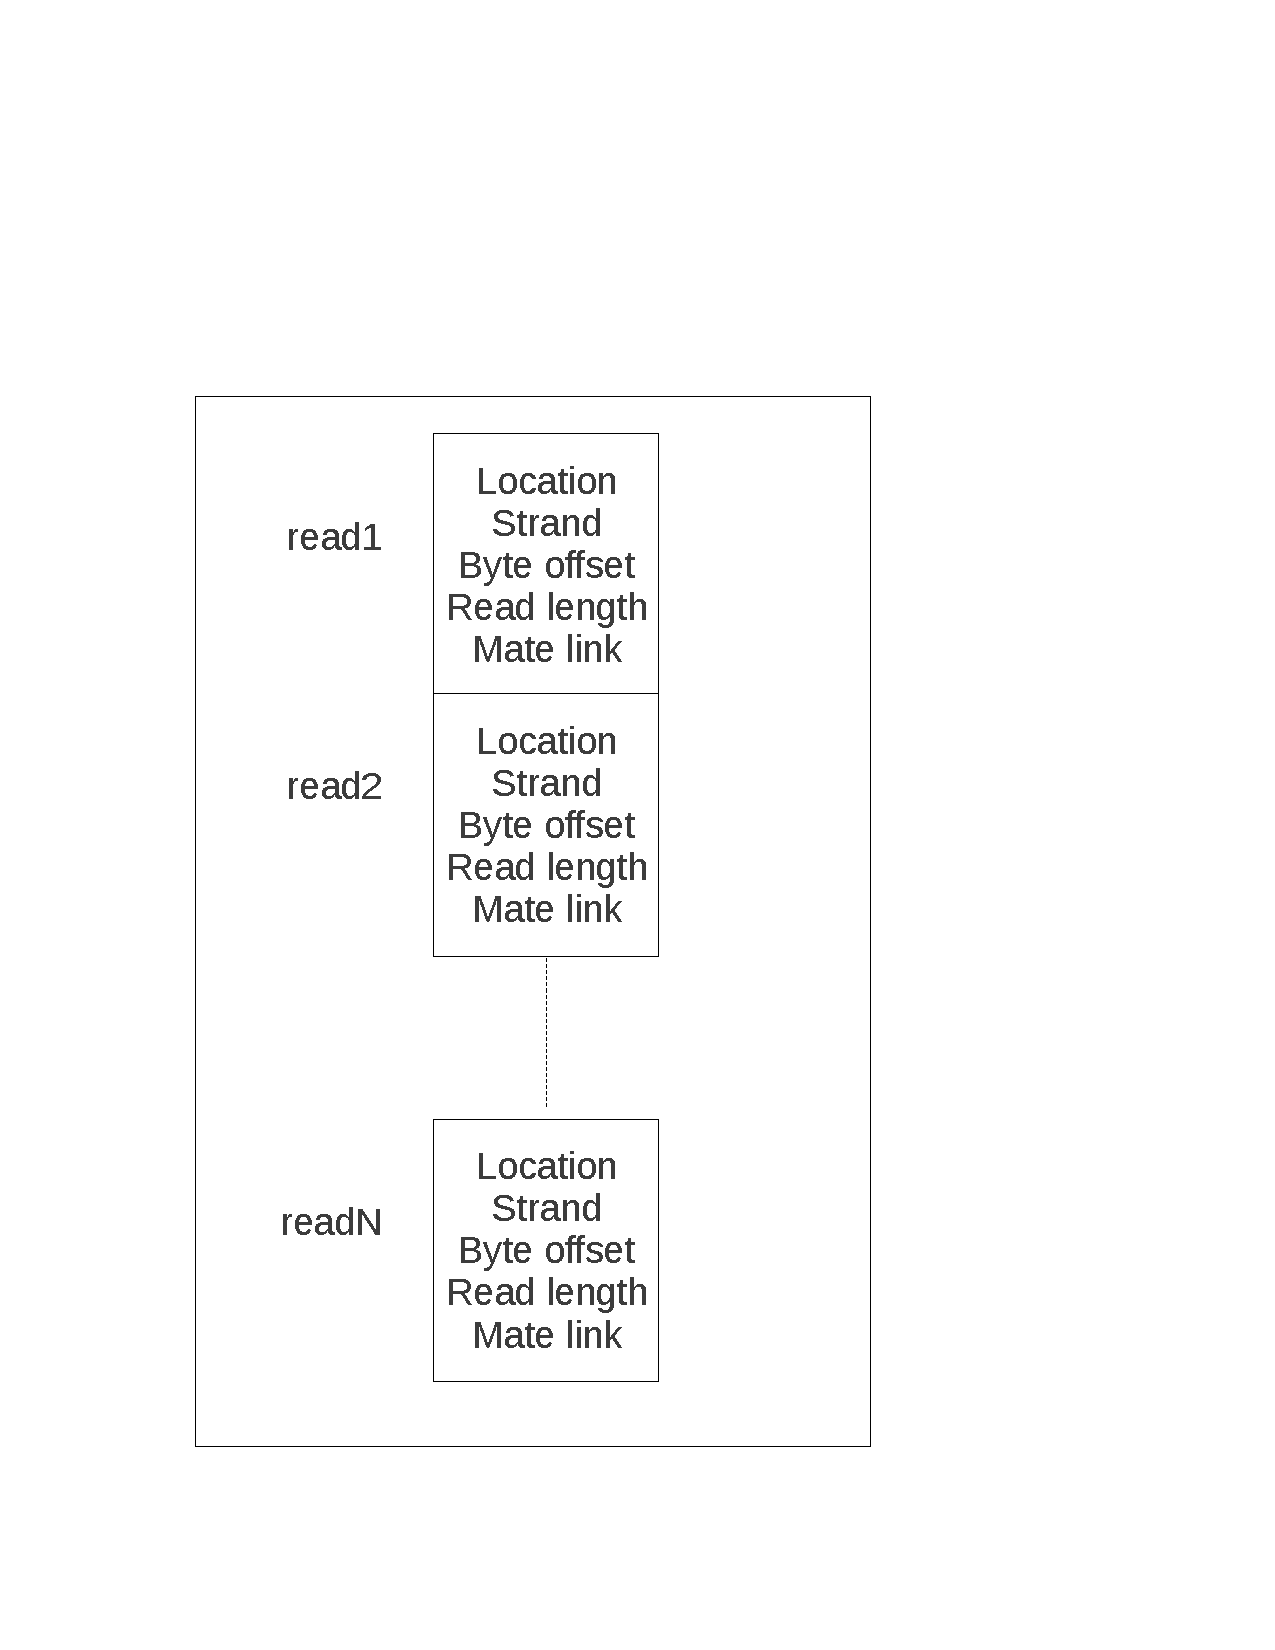
\includegraphics[trim = 30mm 30mm 60mm 40mm,
  clip,width=2in]{fig/indx_descr.pdf}
  \caption{{\footnotesize Our indexing scheme }}
  \label{fig:indx-descr}
\end{figure}


We claim that our index is small enough to fit in the main memory of
any computer. Since we use 8 bytes for the byte offset, 4 bytes for
the mapping location and the mate link, 10 bits for the read length
and 1 bit for the strand information, the size of the index of the set of
alignments of the largest chromosome (chr1) of coverage $35\times$ and
read length of $100$ is $1.5GB$. 

The building of the index occurrs in a small time frame. In our
experiments, a dataset of approximately $90M$ reads from NA18507 
that map with chr1 requires $6$ minutes to create the index, while the
memory footprint of the execution does not exceed $2GB$

\subsection{Read Selection}
\label{sec:read-select}

The size of the index makes the implementation of read selection
straightforward. Since the index of an entire chromosome fits into the
main memory, the selection operation iterates over the index and keeps
the pointers of the reads that satisfy a condition.

\subsection{Read Projection}
\label{sec:read-project}

{\bf TODO: Do we have anything to say here??? we usually type select
* as we always create bam files in the output}.

\subsection{Selection on Interval}
\label{sec:select-int}
{\bf TODO: Need to make clear that we are talking about coverage query
here}


A conventional way of implementing the module that looks for the
maximum interval under a read coverage constraint is an array of
counters for each chromosome coordinate which keep the number
of intervals that include the respective location. The example of
\fref{fig:coverage-example} shows the contents of the counters in an
imaginary scenario of a chromosome of length $10$ and reads of length
$2$. The value of each counter is the number of reads that overlap with 
its location. 

\begin{figure}[hbt]
  \centering
  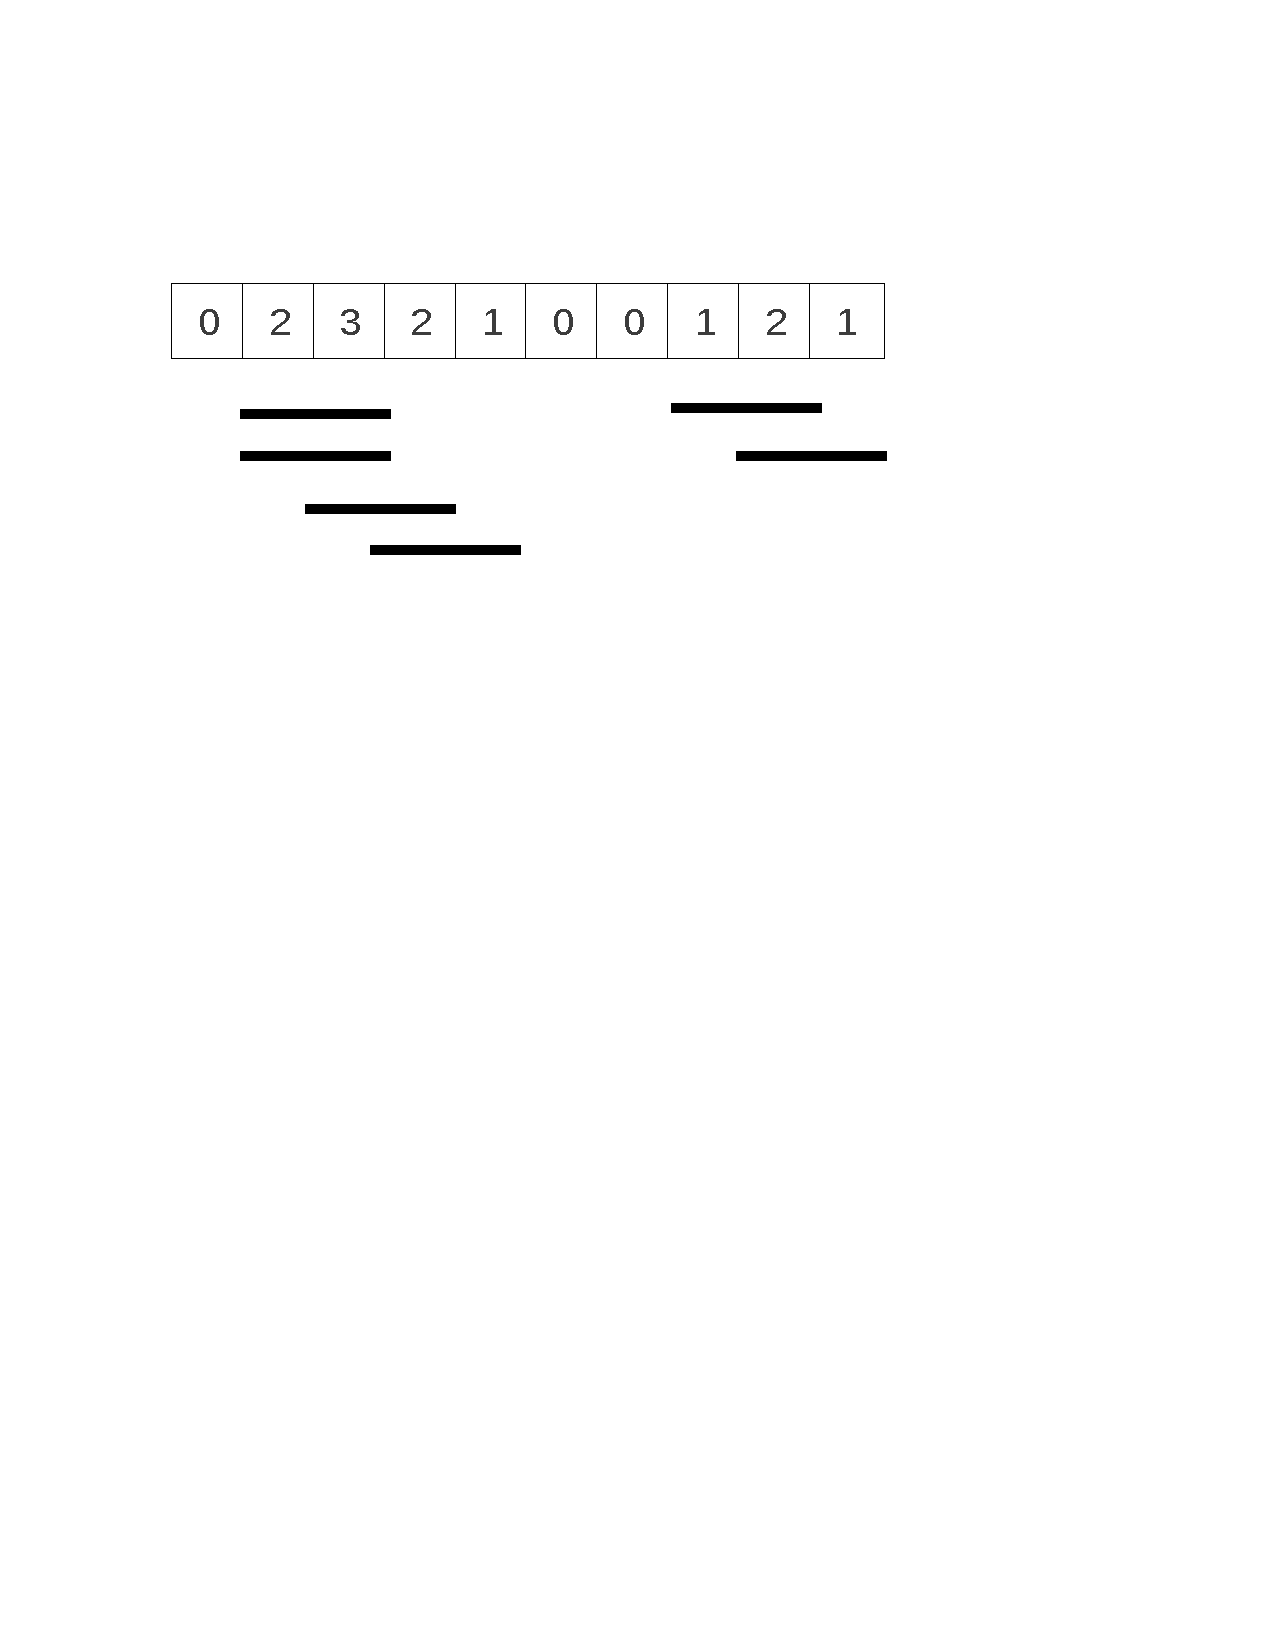
\includegraphics[trim = 15mm 185mm 60mm 40mm,clip,width=2in]{fig/coverage_example.pdf}
  \caption{{\footnotesize The auxiliary vector of counters of a
  selection on intervals.}}
  \label{fig:coverage-example}
\end{figure}

However the linear update of the array of the counters is a computationally
expensive task, because each interval updates as many counters as its
range. Thus, for a chromosome of length $L$, a set of $n$ intervals
each of which has a worst case range $L$, the number of times that counters
need to be updated is $O(n \times L^2)$, where $L$ in the human genome
can be up to $250M$

A more efficient implementation of this module is to model it after
the balanced parenthesis problem. A left parenthesis is assigned for
every opening of an interval and a closing parenthesis is assigned for
every closing of an interval.  Thus the area that is covered by at
least $k$ intervals is the area where $k$ or more parenthesis are open
concurrently. The solution requires a counter which increases each
time a parenthesis is open and decreases when a parenthesis closes.
The regions of interest are the areas for which the values of the
counter are at least $k$.  Now the number of the counter updates that are
required by this algorithm is equal to the number of of the input set
of intervals $n$.

As an example consider the intervals of
\fref{fig:disc-example-a}. \fref{fig:disc-example-b} shows the modeling
of the same intervals with the use of parenthesis. Note that a
parenthesis opens at every position which is the starting point of an
interval and it closes at those positions that are the closing ends of
intervals. The values of the counter appear in the bottom of this figure
and for $k=3$ the area of interest includes all positions whose value
is greater than $2$.

\begin{figure}[hbt]
  \centering
  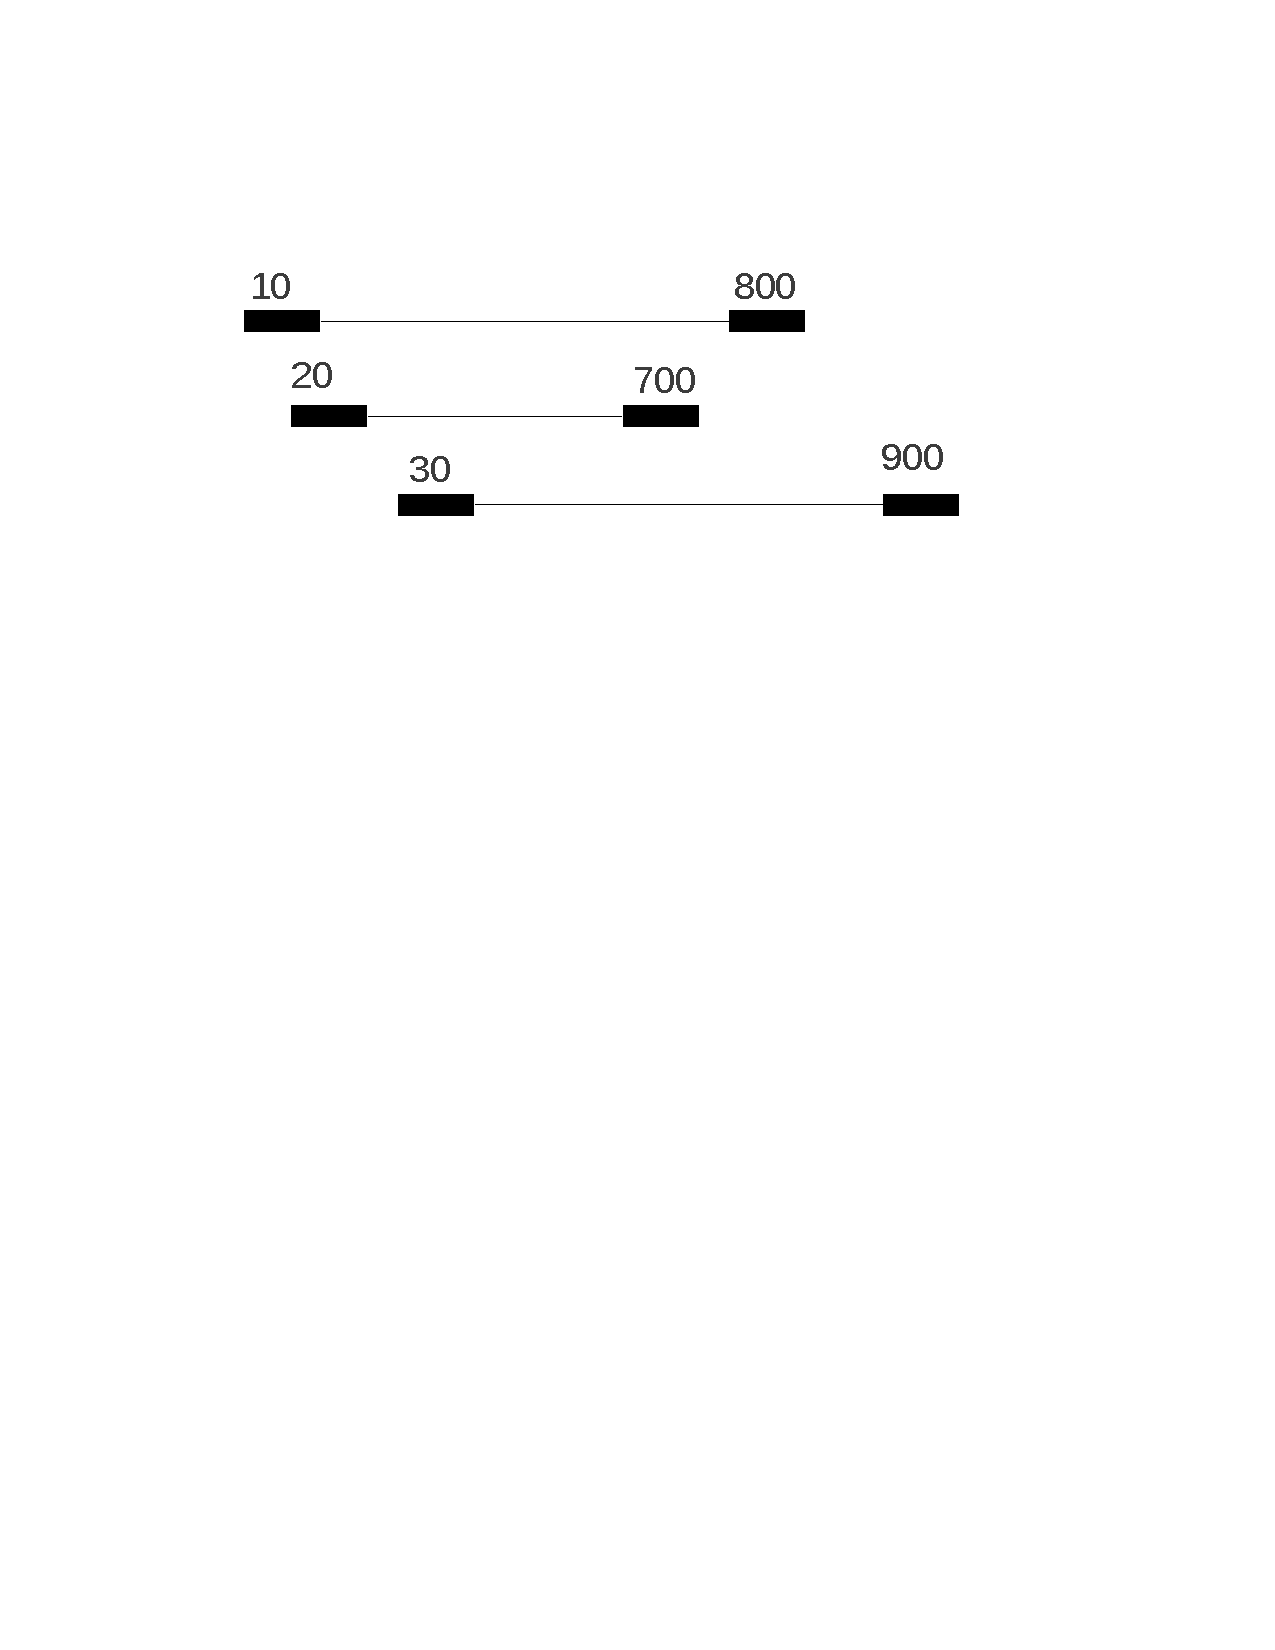
\includegraphics[trim = 30mm 190mm 55mm 40mm,
  clip,width=2in]{fig/disc_example_a.pdf}
  \caption{{\footnotesize A set of intervals.}}
  \label{fig:disc-example-a}
\end{figure}

\begin{figure}[hbt]
  \centering
  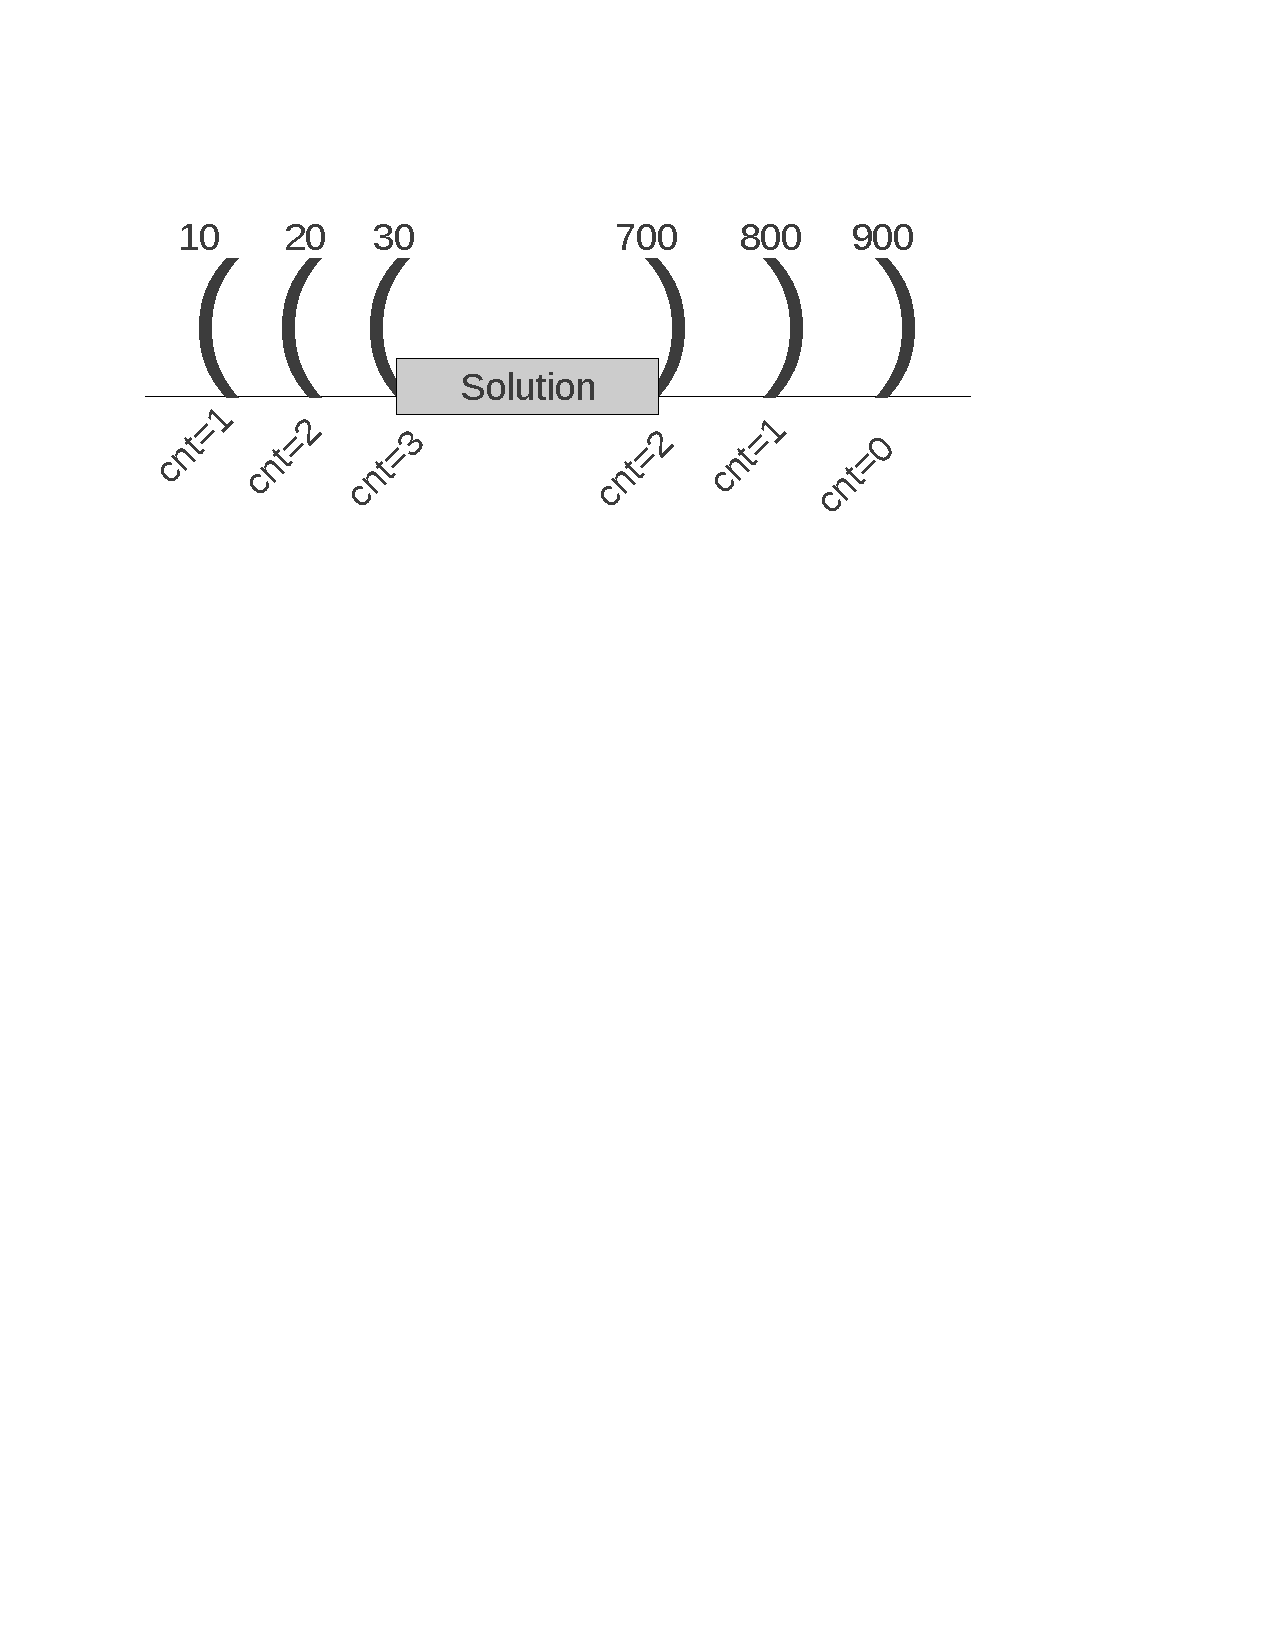
\includegraphics[trim = 25mm 190mm 55mm 30mm,
  clip,width=2in]{fig/disc_example_b.pdf}
  \caption{{\footnotesize The intervals are modeled as
  parenthesis. The shaded area is the region which is covered by at
  least $3$ intervals.}}
  \label{fig:disc-example-b}
\end{figure}


\subsection{Mapjoin}
\label{sec:mapjoin}
Following the lead of \cite{nclist}, the implementation of the {\em Mapjoin} 
between two tables requires the use of interval trees. We create an
interval tree on the table with the smallest set of intervals and we
query it with each interval of the largest one. From the matching
intervals we generate tuples of pointers, one from each table, that
represent the join of the fields that intersect.



\section{Visualization}
\label{sec:gui}

\section{Results}
\label{sec:results}

The database of our experiments consists of genome NA18507
\cite{Altshuler05} which is the output of the sequencing of a male person
from Yoruba in Ibadan, Nigeria that has been conducted in the context
of the 1000-Genomes project \cite{Durbin2010} using Illumina's latest
mate pair based sequencing technology. The data consist of
$1176090451$ reads of length $100$ which is a yield of a genome
coverage of $40\times$ and the size of the BAM file that
stores the reads is $73$GB. The alignment of the reads has been done
against version hg18 of the human reference \cite{hg18} using
Eland, Illumina's propietary alignment tool. $1104952383$ of the reads
have been mapped. $1033814315$ of the mapped reads have their mate
also mapped and the rest $71138068$ are singletons. $5832322$ of the
mapped reads have their mate mapped to a different chromosome.

\subsection{A few challenging queries}
\label{sec:self}

\paragraph{Get the evidence of all isolated deleted regions}

The evidence of the deleted regions comes from the observation that
the distance between the alignments of the reads of a pair is
unjustifiably large. To eliminate outlying information we require that
an area to be deleted needs to be supported by at least 3 different
clones. \fref{alg:deletion-gql} shows the gql code of the query which
needs $369$seconds to run and returns $226011$ reads. 

\begin{algorithm}
\begin{lstlisting}[firstline=2,breaklines=true]
use parsed_tables
import READS;

H1=select create_intervals() 
from READS using intervals (location,mate_loc,both_mates) 
where location>=0 and 
mate_loc>=0 and 
(
(mate_loc-location>1000 and mate_loc-location<100000) or (location-mate_loc>1000 and location-mate_loc<100000)
)

select merge_intervals(interval_coverage>3) from H1
\end{lstlisting}
\caption{{\footnotesize The gql code of the deletion query.}}
\label{alg:deletion-gql}
\end{algorithm}

%\begin{figure}[hbt]
%  \centering
%  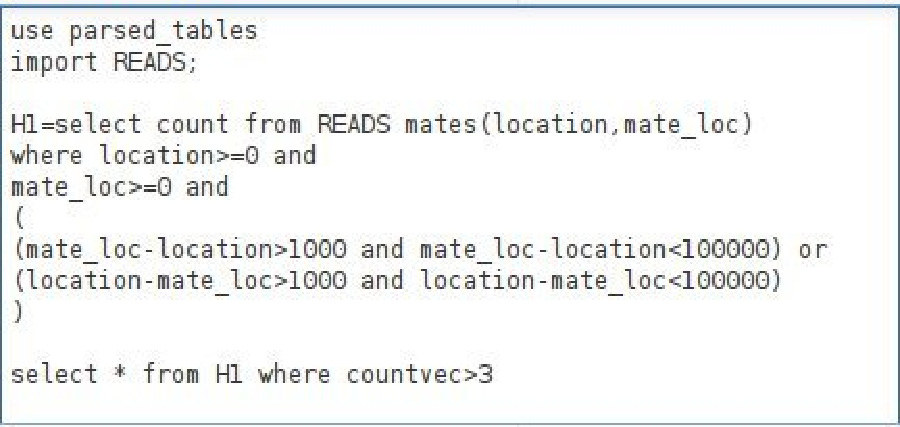
\includegraphics[trim = 0mm 0mm 0mm 0mm,
%  clip,width=2in]{fig/deletion_gql.pdf}
%  \caption{{\footnotesize The gql code of the deletion query.}}
%  \label{fig:deletion-gql}
%\end{figure}

\paragraph{Get the evidence of all inverted regions}

The evidence of the inverted regions comes from the observation that
the orientation of the involved clones is inverted. In Illumina
sequencing, normal clones are expected to such that the ``leftmost''
end of a pair maps with the forward strand while the ``rightmost'' end
maps with the reverse strand. Thus the query that is shown in
\fref{alg:inversion-gql} looks for regions that are covered by at
least 5 different pairs of reads where the leftmost end of each pair
maps with the reverse strand and the rightmost end maps with the
forward strand. The query needs $476$ seconds to run and returns
$202632$ reads.

\begin{algorithm}
\begin{lstlisting}[firstline=2,breaklines=true]
use parsed_tables
import READS;

H1=select create_intervals() 
from READS using intervals (location,mate_loc, both_mates) 
where location>=0 and 
mate_loc>=0 and 
(
( mate_loc>location and strand=='-' and mate_strand=='+') or
( location>mate_loc and strand=='+' and mate_strand=='-')
)


select merge_intervals(interval_coverage>5) from H1
\end{lstlisting}
\caption{{\footnotesize The gql code of the inversion query.}}
\label{alg:inversion-gql}
\end{algorithm}
%\begin{figure}[hbt]
%  \centering
%  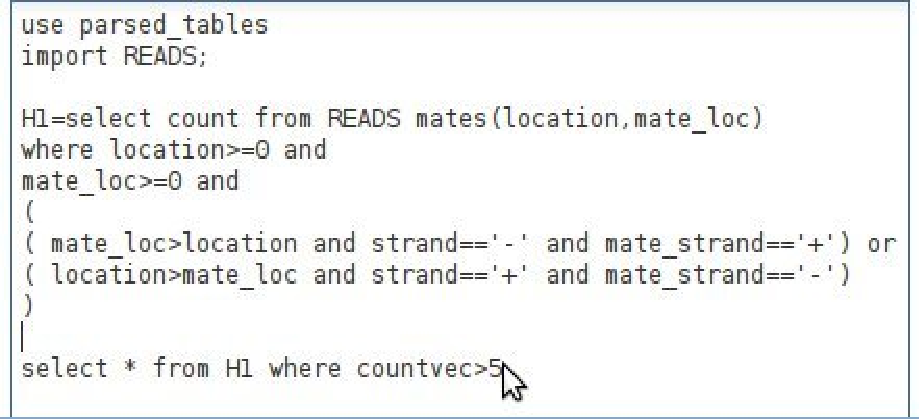
\includegraphics[trim = 0mm 0mm 0mm 0mm,
%  clip,width=2in]{fig/inversion_gql.pdf}
%  \caption{{\footnotesize The gql code of the inversion query.}}
%  \label{fig:inversion-gql}
%\end{figure}


\paragraph{Find all regions with high copy number}

Regions that are covered by unrealistically large numbers of reads are
called high copy number regions. Normally, the number of reads that are
expected to be found in a region is equal to the coverage of the
experiment, which in our datasets is $40$. Thus the query that is
shown in \algref{alg:highcnv-gql} looks for regions that are covered by
at least $200$ reads. The query needs $2141$ seconds to run and the
evidence data of the output consist of $10979437$ reads.

\begin{algorithm}
\begin{lstlisting}[firstline=2,breaklines=true]
use parsed_tables
import READS;

H1=select create_intervals() 
from READS
where location>=0 

select merge_intervals(interval_coverage>200) from H1 
\end{lstlisting}
\caption{{\footnotesize The gql code of the high copy number query.}}
\label{alg:highcnv-gql}
\end{algorithm}

%\begin{figure}[hbt]
%  \centering
%  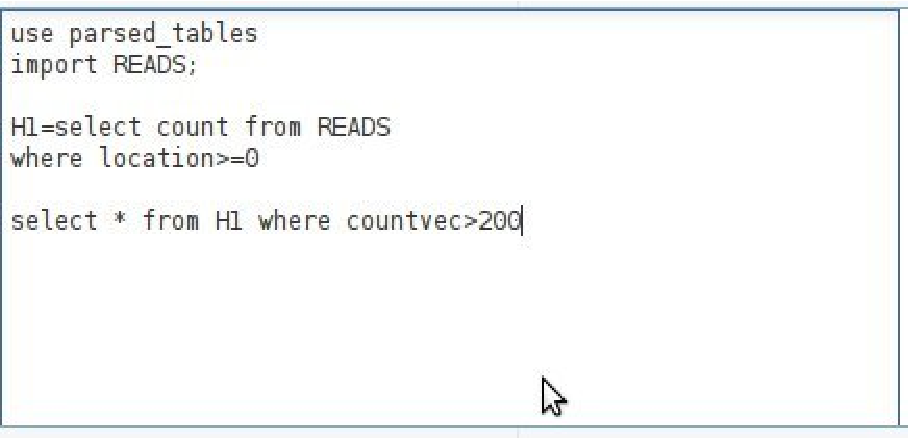
\includegraphics[trim = 0mm 0mm 0mm 0mm,
%  clip,width=2in]{fig/highcnv_gql.pdf}
%  \caption{{\footnotesize The gql code of the high copy number query.}}
%  \label{fig:highcnv-gql}
%\end{figure}



\paragraph{Get all reads and their mates that overlap with some gene}

The query uses an external table which consists of all known genes
according to the RefSeq database. The output of this query is the
mapjoin of all mapped reads with the coordinates of the UCSC database.
\fref{alg:genecoverage-gql} shows the gql syntax of the query which
needs $17311$seconds to run and returns $495454218$ reads. Note that the large
execution time of the query is bounded by the IO. To verify that, we
utilized samtools, which provide an extremely efficient indexing
scheme for range retrieval, to fetch the same ranges of reads. It took
samtools $19875$seconds to fetch the same ranges of data which is even slower. 

\begin{algorithm}
\begin{lstlisting}[firstline=2, breaklines=true]
use parsed_tables
import READS;
import genes;

H2=select * from READS where location>0

H3=select * 
from MAPJOIN genes using intervals(begin, end),H2 using intervals (location, location+length, both_mates)

select * from H3 
where location>0
\end{lstlisting}
\caption{{\footnotesize The gql code that retrieves all reads and
  their mates that overlap with some gene.}}
\label{alg:genecoverage-gql}
\end{algorithm}

%\begin{figure}[hbt]
%  \centering
%  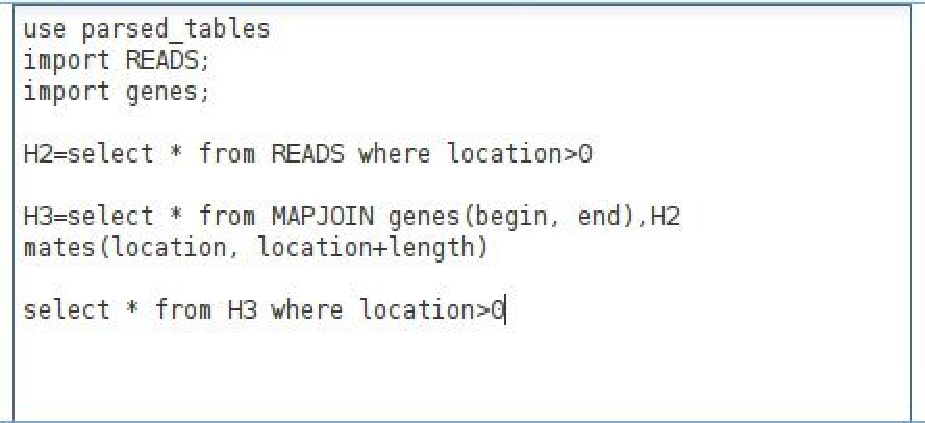
\includegraphics[trim = 0mm 0mm 0mm 0mm,
%  clip,width=2in]{fig/genecoverage_gql.pdf}
%  \caption{{\footnotesize The gql code that retrieves all reads and
%  their mates that overlap with some gene.}}
%  \label{fig:genecoverage-gql}
%\end{figure}



\subsection{Integration with known software}
\label{sec:integration}


%\end{document}  % This is where a 'short' article might terminate

% ensure same length columns on last page (might need two sub-sequent latex runs)
\balance

\section{Acknowledgments}

\bibliographystyle{abbrv}
\bibliography{query}  % vldb_sample.bib is the name of the Bibliography in this case



\end{document}
